\section{Klassen}
    TODO Bild eines vereinfachten Modells

    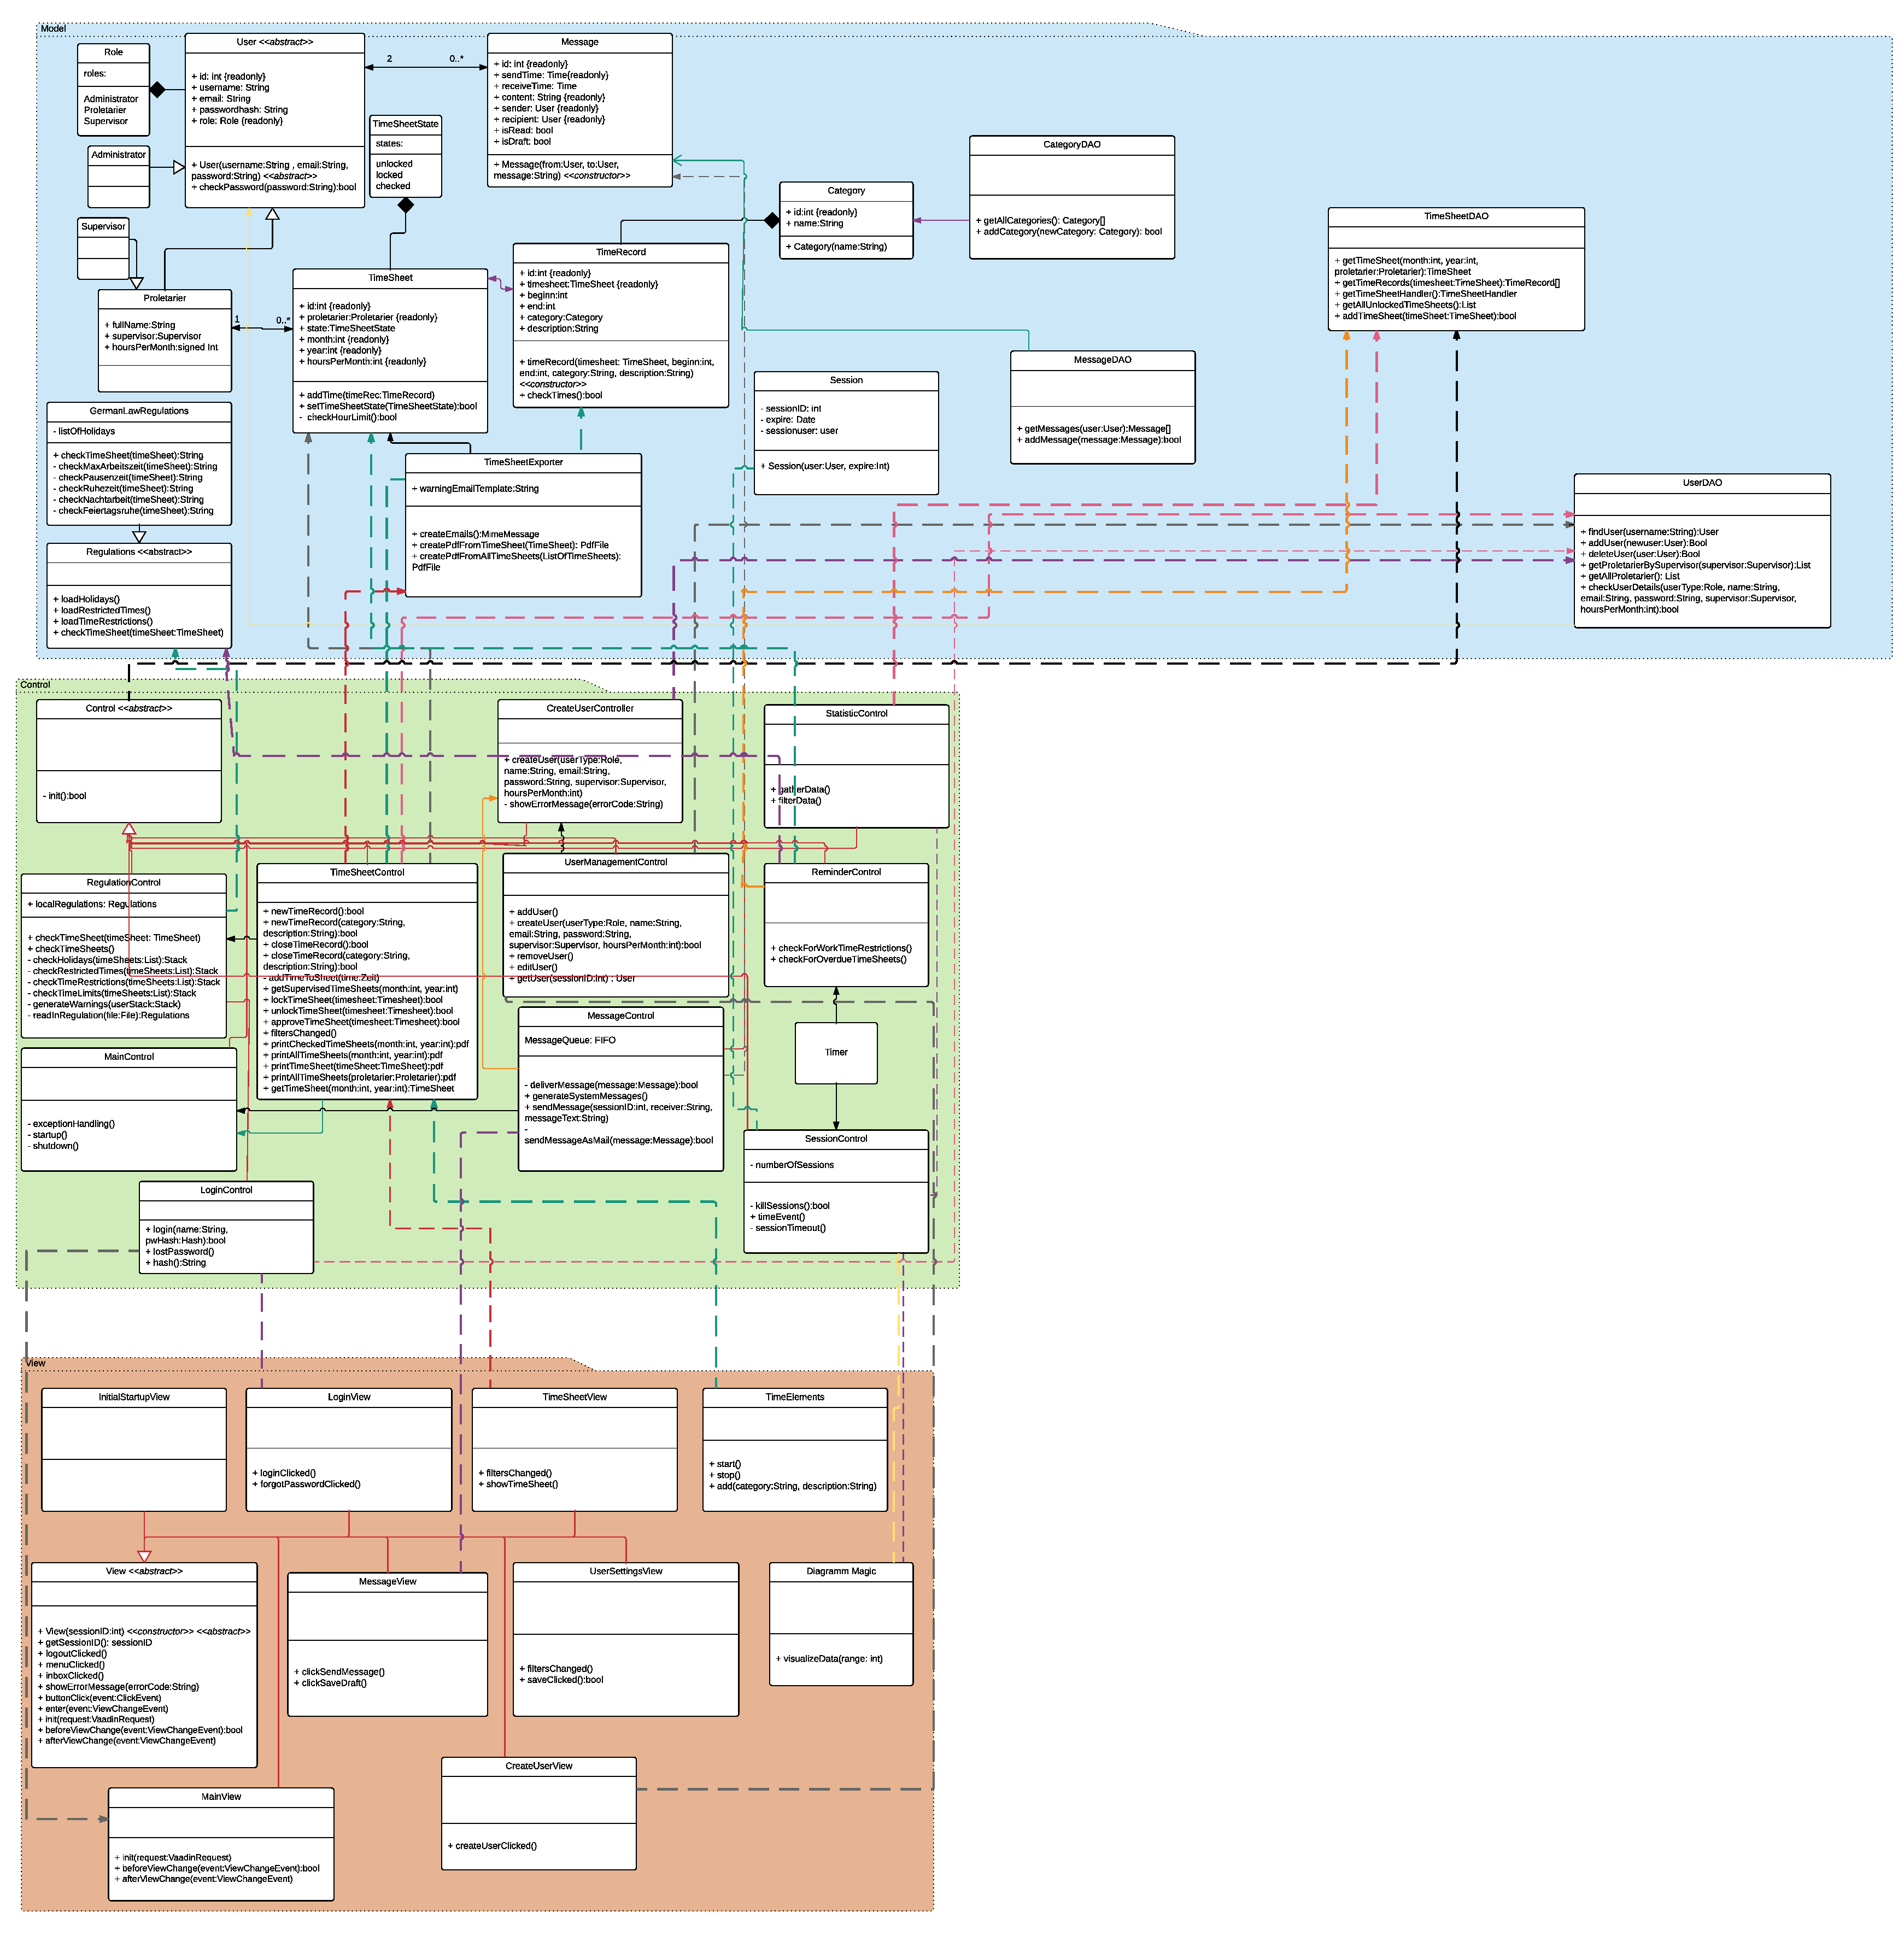
\includegraphics[width=\linewidth]{Diagramms/class/overview.pdf}\\
    TODO Bild des kompletten Klassendiagrams (ggf ans ende/in den anhang?)
    \newpage
    \subsection{Model}
        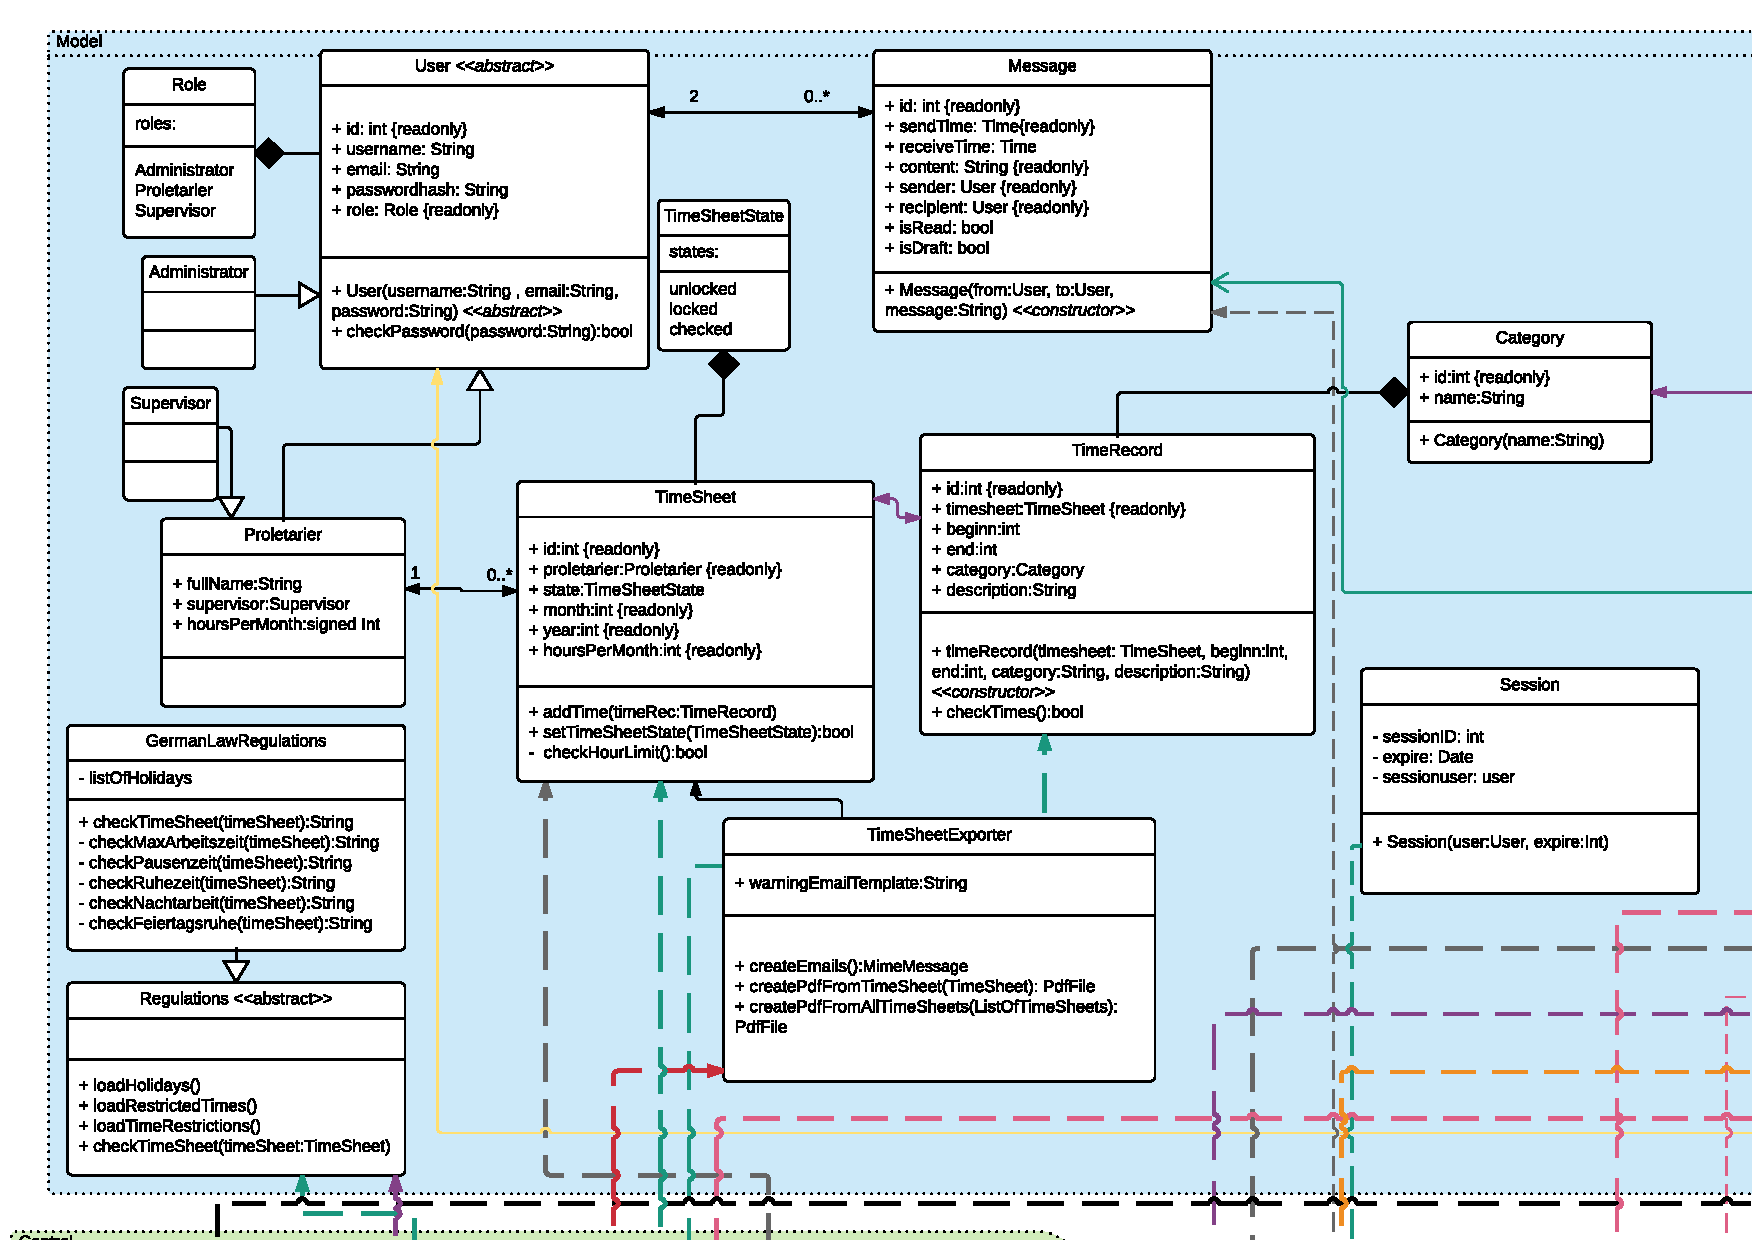
\includegraphics[width=\linewidth,page=1]{Diagramms/class/model.pdf}\\
        \includegraphics[width=\linewidth,page=2]{Diagramms/class/model.pdf}\\
        \begin{itemize}
            \itm{User}
                Grundform eines Benutzers, stellt grundlegende Daten und Funktionen für spezialisierte Benutzer bereit.
                Es gibt folgende Spezialisierungen: Administrator, Proletarier und Supervisor.

                \emph{Attribute:}
                \begin{itemize}
                    \itm{id:int}
                        Autogenerierte, von der Datenbank vergebene ID.
                        Kann nicht verändert werden.
                    \itm{username:String}
                        Benutzername der das Einloggen vereinfachen soll.
                        Kann nur vom User eingesehen und geändert werden.
                    \itm{email:String}
                        Eine Email-Adresse des Users.
                        Wird genutzt um den User zu kontaktieren.
                        Kann nur vom User oder einem Administrator eingesehen und geändert werden.
                    \itm{passwordhash:String}
                        Ein kryptographischer, gesalzener Hash des Passworts.
                        Kann nur vom User oder einem Administrator geändert und von niemandem eingesehen werden.
                    \itm{role:Role}
                        Die Rolle des Users.
                        Kann nur implizit vom Programm zwischen User und Supervisor geändert werden, je nachdem ob der User irgendwo als Supervisor eingetragen ist und selbst einen Supervisor hat.
                        Kann vom User und Administratoren eingesehen werden.
                \end{itemize}
                \emph{Methoden:}
                \begin{itemize}
                    \itm{User(username:String , email:String, password:Hash)}
                    \itm{checkPassword(password:Hash):bool}
                        Gibt true zurück wenn das Passwort korrekt ist sonst false.
                \end{itemize}

            \itm{Administrator}
                Stellt Daten für und über den Administrator bereit.
                Der Administrator verwaltet die anderen User, kann jedoch selbst keinen Stundenzettel führen.


            \itm{Proletarier}
                Stellt Daten für und über den Proletarier bereit, darüber hinaus hat der Proletarier eine Verbindung zu dem mit ihm assozierten Zeiterfassungen und Stundenzetteln.

                \emph{Attribute:}\\
                Alle Attribute können nur vom Proletarier, dem entsprechenden Supervisor oder einem Administrator eingesehen werden.
                \begin{itemize}
                    \itm{fullName:String}
                        Der volle Name der später auf dem Stundenzettel steht.
                        Kann nur vom Proletarier oder einem Administrator geändert werden.
                    \itm{supervisor:Supervisor}
                        Der Supervisor des Proletariers.
                        Kann nur von einem Administrator geändert werden.
                    \itm{hoursPerMonth:int}
                        Die Stunden die pro Monat gearbeitet werden müssen.
                        Kann nur von einem Administrator geändert werden.
                \end{itemize}

            \itm{Supervisor}
                Erweiterung des Proletarier um Gruppen von Usern zu verwalten.
                Hat sich selbst als Supervisor.

            \itm{TimeSheet}
                Speichert Zeiterfassungen. Methoden zur Validierung und Sicherstellung der Unveränderlichkeit sind vorhanden.
                
                \emph{Attribute:}
                \begin{itemize}
                    \itm{id:int}
                        Autogenerierte, von der Datenbank vergebene ID.
                        Kann nicht verändert werden.
                    \itm{proletarier:Proletarier}
                        Gibt an, zu welchem Proletarier dieser Stundenzettel gehört.
                        Wird beim Erstellen gesetzt und kann nicht geändert werden.
                    \itm{state:TimeSheetState}
                        Gibt den aktuellen Status des Stundenzettels an.
                        Mögliche Zustände sind: unlocked, locked, checked.
                        Kann vom Proletarier oder dessen Supervisor von unlocked zu locked geändert werden.
                        Kann nur vom zugehörigen Supervisor von locked zu unlocked oder checked verändert werden.
                        Kann nur von Administratoren von checked in etwas anderes geändert werden.
                    \itm{month:int}
                        Gibt den Monat an, für den der Stundenzettel gilt.
                        Wird beim Erstellen gesetzt und kann nicht geändert werden.
                    \itm{year:int}
                        Gibt das Jahr an, für das der Stundenzettel gilt.
                        Wird beim Erstellen gesetzt und kann nicht geändert werden.
                    \itm{hoursPerMonth:int}
                        Gibt an, wieviele Stunden in diesem Monat gearbeitet werden müssen.
                        Wird beim Erstellen gesetzt und kann nicht geändert werden.
                \end{itemize}
                \emph{Methoden:}
                \begin{itemize}
                    \itm{addTime(timeRec:TimeRecord)}
                    \itm{setTimeSheetState(TimeSheetState):bool}
                    \itm{checkHourLimit():bool}
                \end{itemize}

            \itm{TimeRecord}
                Datenhaltung, der Zeiterfassung.
                \emph{Attribute:}
                \begin{itemize}
                    \itm{id:int}
                        Autogenerierte, von der Datenbank vergebene ID.
                        Kann nicht verändert werden.
                    \itm{timesheet:TimeSheet}
                        Gibt an, zu welchem Stundenzettel diese Zeiterfassung gehört.
                        Wird beim Erstellen gesetzt und kann nicht geändert werden.
                    \itm{beginn:int}
                        Gibt an, zu welchem Zeitpunkt die Zeiterfassung gestartet wurde.
                        Die Zeit wird als Unix time gespeichert und auf Minuten gerundet.
                        Kann nur vom Proletarier verändert werden.
                        Kann nur vom Proletarier, dem entsprechenden Supervisor und Administratoren eingesehen werden.
                    \itm{end:int}
                        Gibt an, zu welchem Zeitpunkt die Zeiterfassung beendet wurde.
                        Die Zeit wird als Unix time gespeichert und auf Minuten gerundet.
                        Kann nur vom Proletarier verändert werden.
                        Kann nur vom Proletarier, dem entsprechenden Supervisor und Administratoren eingesehen werden.
                    \itm{category:Category}
                        Gibt an, in welche Kategorie die Tätigkeit fällt.
                        Kann nur vom Proletarier verändert werden.
                        Kann nur vom Proletarier, dem entsprechenden Supervisor und Administratoren eingesehen werden.
                    \itm{description:String}
                        Gibt eine kurze Beschreibung der Tätigkeit an.
                        Kann nur vom Proletarier verändert werden.
                        Kann nur vom Proletarier, dem entsprechenden Supervisor und Administratoren eingesehen werden.
                \end{itemize}
                \emph{Methoden:}
                \begin{itemize}
                   \itm{timeRecord(timesheet: TimeSheetbeginn:int, end:int, category:String, description:String)}
                   \itm{checkTimes():bool}
                \end{itemize}

            \itm{TimeSheetExporter}
                \emph{Attribute:}
                \begin{itemize}
                    \itm{warningEmailTemplate:String}
                        Die Vorlage für die Email die verschickt wird, wenn Proletarier ihren Stundenzettel des letzten Monats noch nicht fertiggestellt haben.
                        Kann nur von Administratoren eingesehen und geändert werden.
                \end{itemize}
                \emph{Methoden:}
                \begin{itemize}
                    \itm{setTimeSheetState(TimeSheet, TimeSheetState):bool}
                    \itm{createPdfFromTimeSheet(TimeSheet): PdfFile}
                    \itm{createPdfFromAllTimeSheets(ListOfTimeSheets): PdfFile}
                \end{itemize}

            \itm{Category}
                Kategorie, die für die Zeiterfassung benötigt wird
                \emph{Attribute:}
                \begin{itemize}
                    \itm{id:int}
                        Autogenerierte, von der Datenbank vergebene ID.
                        Kann nicht verändert werden.
                    \itm{name:String}
                        Der Name einer Kategorie.
                        Kann von allen eingesehen, jedoch nur von Administratoren geändert werden.
                \end{itemize}
                \emph{Methoden:}
                \begin{itemize}
                    \itm{Category(name:String)}
                \end{itemize}

            \itm{Message}
                Nachrichten und damit verbundene Metadaten können mit dieser Klasse erfasst werden.
                \emph{Attribute:}
                \begin{itemize}
                    \itm{id:int}
                        Autogenerierte, von der Datenbank vergebene ID.
                        Kann nicht verändert werden.
                    \itm{sendTime:int}
                        Die Uhrzeit zu der die Nachricht gesendet wurde.
                        Die Zeit wird als Unix time gespeichert und auf Minuten gerundet.
                        Wird beim Erstellen gesetzt und kann nicht geändert werden.
                    \itm{receiveTime:int}
                        Die Uhrzeit zu der die Nachricht vom Empfänger gelesen wurde.
                        Die Zeit wird als Unix time gespeichert und auf Minuten gerundet.
                        Kann nur vom empfangenden Proletarier eingesehen und geändert werden.
                    \itm{content:String}
                        Der Inhalt der Nachricht.
                        Wird beim Erstellen gesetzt und kann nicht geändert werden.
                    \itm{sender:User}
                        Der User der die Nachricht schickt oder in dessen Namen die Nachricht geschickt wird.
                        Dieses Feld kann leer sein, falls das System die Nachricht geschickt hat.
                        Wird beim Erstellen gesetzt und kann nicht geändert werden.
                    \itm{recipient:User}
                        Der Empfänger der Nachricht.
                        Wird beim Erstellen gesetzt und kann nicht geändert werden.
                    \itm{isRead:bool}
                        Ob der Empfänger die Nachricht bereits gelesen hat.
                        Kann nur vom empfangenden Proletarier eingesehen und geändert werden.
                \end{itemize}
                \emph{Methoden:}
                \begin{itemize}
                    \itm{Message(from:User, to:User, message:String)}
                \end{itemize}

            \itm{UserDAO}
                Listet alle vorhanden User auf. Enthält Methoden um User hinzuzufügen, zu löschen oder zu verändern. Stellt darüber hinaus sicher, dass die alle Einträge einzigartig sind.
                \emph{Methoden:}
                \begin{itemize}
                   \itm{findUser(username:String):User}
                   \itm{addUser(newEntity:User):Bool}
                       Gibt true zurück wenn die User erstellt werden konnte.
                       False bei Fehler.
                   \itm{deleteUser(User:User):Bool}
                       Gibt true zurück wenn die User gelöscht werden konnte.
                       False bei Fehler.
                   \itm{checkCredentials(userName:String, pwHash:Hash):Bool}
                       Gibt true zurück wenn Username und Passwort korrekt sind, sonst false.
                   \itm{getProletarierBySupervisor(supervisor:Supervisor):List}
                   \itm{getAllProletarier(): List}
                   \itm{checkUserDetails(userType:Role, name:String, email:String, password:String, supervisor:Supervisor, hoursPerMonth:int):bool}
                \end{itemize}

            \itm{TimeSheetDAO}
                Listet alle TimeSheets.
                \emph{Methoden:}
                \begin{itemize}
                    \itm{getTimeSheet(month:int, year:int, proletarier:Proletarier):TimeSheet}
                    \itm{getTimeRecords(timesheet:TimeSheet):TimeRecord[]}
                    \itm{getTimeSheetHandler():TimeSheetHandler}
                    \itm{getAllUnlockedTimeSheets():List}
                    \itm{addTimeSheet(timeSheet:TimeSheet):bool}
                \end{itemize}

            \itm{CategorieDAO}
                Liste aller verfügbaren Kategorien.
                \emph{Methoden:}
                \begin{itemize}
                   \itm{getAllCategories(): Category[]}
                   \itm{addCategory(newCategory: Category): bool}
                \end{itemize}

            \itm{MessageDAO}
                Nachrichten und damit Verbundene Metadaten können mit dieser Klasse erfasst werden.
                \emph{Methoden:}
                \begin{itemize}
                    \itm{getMessages(user:User):Message[]}
                    \itm{addMessage(message:Message):bool}
                \end{itemize}

            \itm{Regulations}
                Lädt die gesetzlichen Regularien aus einer Datei und stellt diese für andere Klassen bereit.
                \emph{Methoden:}
                \begin{itemize}
                    \itm{loadHolidays()}
                    \itm{loadRestrictedTimes()}
                    \itm{loadTimeRestrictions()}
                \end{itemize}

            \itm{GermanLawRegulations}
                Lädt die gesetzlichen Regularien aus einer Datei und stellt diese für andere Klassen bereit.\\
                \emph{Attribute:}
                    \begin{itemize}
                        \itm{listOfHolidays}
                    \end{itemize}


            \itm{TimeSheetState}
                Zustände, die beschreiben, ob ein Stundenzettel verändert werden darf, bzw bereits überprüft wurde.
                Mögliche Zustände:
                \begin{itemize}
                    \itm{unlocked}
                        Der Time Sheet kann bearbeitet werden.
                    \itm{locked}
                        der Time Sheet ist abgeben worden und es deshalb gegen bearbeitung gesperrt.
                    \itm{checked}
                        Der Time Sheet wurde vom Supervisor überprüft.
                \end{itemize}

            \itm{Session}
                Daten die mit einer Login Session assoziert sind(Proletarier, Ablaufdatum, ...) werden in dieser Klasse gespeichert.
                \begin{itemize}
                    \itm{Session(User:User, expire:Int)}
                \end{itemize}


        \end{itemize}

    \subsection{Control}
        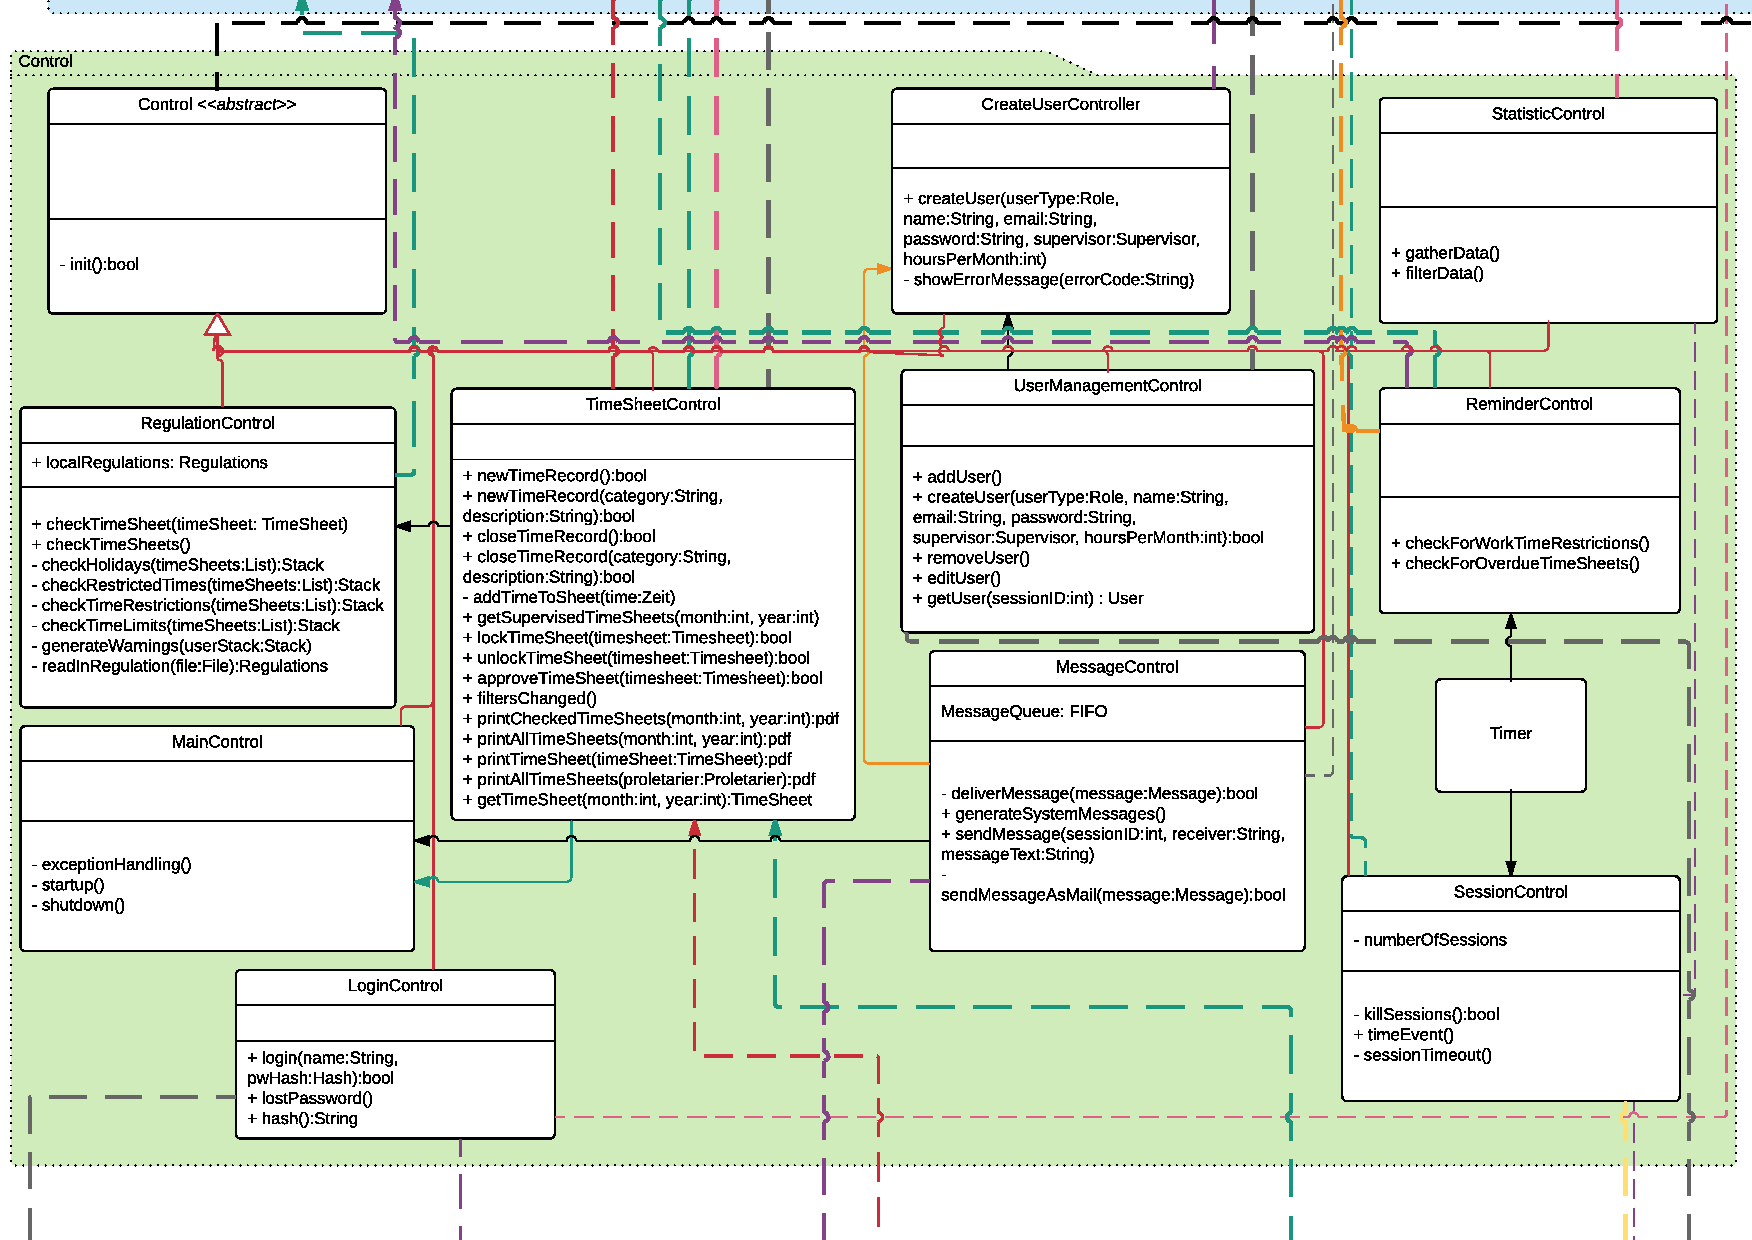
\includegraphics[width=\linewidth]{Diagramms/class/control.pdf}\\
        \begin{itemize}
            \itm{Control}
            \item Jede von Control erbende Klasse implementiert das Einzelstück-Entwurfsmuster, da die Control-Klassen keinen Zustand benötigen.
                \emph{Methoden:}
                \begin{itemize}
                    \item{init():bool}
                        Das Initialisierungsablauf jeder Klasse
                \end{itemize}
                \emph{Erbende Klassen:}
                \begin{itemize}
                    \itm{RegulationControl}
                       Überprüft Daten auf Gesetzeskonformität, leitet ebenfalls notwendige Schritte ein.
                       \begin{itemize}
                           \itm{checkRegulations():bool}
                            Es werden erfasste Zeiten auf ihre konformität geprüft.
                            \itm{checkHolidays(timeSheets:List):Stack}
                            \itm{checkRestrictedTimes(timeSheets:List):Stack}
                            \itm{checkTimeRestrictions(timeSheets:List):Stack}
                            \itm{checkTimeLimits(timeSheets:List):Stack}
                            \itm{generateWarnings()}
                            Erzeugt Messages über Verletzungen der Regularien.
                            \itm{readInRegulation(file:File):Regulations}
                       \end{itemize}

                    \itm{ReminderControl}
                        Überprüft in regelmäßigen abständen, ob Erinnerungen versendet werden müssen.
                        \emph{Methoden:}
                        \begin{itemize}
                            \itm{checkForWorkTimeRestrictions()}
                            \itm{checkForOverdueTimeSheets()}
                        \end{itemize}

                    \itm{MainControl}
                        Kontrolliert den Hauptablauf des Programms.
                        \begin{itemize}
                            \itm{exceptionHandling()}
                                Im Falle von kritischen Excepetions, wird der Dienst gepeichert und runtergefahren.
                            \itm{startup()}
                                Startroutine des Servers.
                            \itm{shutdown()}
                                Abschaltverhalten des Servers.
                        \end{itemize}

                    \itm{TimeSheetControl}
                        Regelt die Erstellung von Stundendaten für den Stundenzettel, darüber hinaus wird auch die Abarbeitung eines fertigen Stundenzettels geregelt.
                        \begin{itemize}
                             \itm{newTimeRecord():bool}
                             \itm{newTimeRecord(category:String, description:String):bool}
                             \itm{closeTimeRecord():bool}
                             \itm{closeTimeRecord(category:String, description:String):bool}
                             \itm{addTimeToSheet(time:Zeit)}
                             \itm{getSupervisedTimeSheets(month:int, year:int)}
                             \itm{lockTimeSheet(month:int, year:int):bool}
                             \itm{filtersChanged()}
                             \itm{printLockedTimeSheets(month:int, year:int)}
                             \itm{getTimeSheet(month:int, year:int):TimeSheet}
                        \end{itemize}

                    \itm{UserManagementControl}
                        Managed das hinzufügen, löschen und verändern von Benutzern
                        \begin{itemize}
                             \itm{addUser()}
                             \itm{createUser(userType:Role, supervisor: Supervisor)}
                             \itm{removeUser()}
                             \itm{editUser()}
                             \itm{getUser(sessionID:int): User}
                        \end{itemize}

                    \itm{LoginControl}
                        Überwacht das korrekte Einloggen von Benutzern.
                        \begin{itemize}
                             \itm{login(name:String, pwHash:Hash):bool}
                             \itm{lostPassword()}
                             \itm{hash():String}
                        \end{itemize}

                    \itm{MessageControl}
                        Stellt Nachrichten zwischen Benutzern (und dem System) zu.
                        \begin{itemize}
                             \itm{deliverMessage(message:Message):bool}
                             \itm{generateSystemMessages()}
                             \itm{sendMessage()}
                             \itm{sendMessageAsMail(message:Message):bool}
                        \end{itemize}

                    \itm{StatisticControl}
                        Sammelt und generiert Statistiken über die erfassten Stundendaten.
                        \begin{itemize}
                             \itm{gatherData()}
                             \itm{filterData()}
                        \end{itemize}

                    \itm{SessionControl}
                        Kontrolliert offene Sessions und terminiert diese nach ablauf eines gesetzen Zeitraums.
                        \begin{itemize}
                            \itm{killSessions():bool}
                            \itm{timeEvent()}
                            \itm{sessionTimeout()}
                        \end{itemize}
                \end{itemize}

            \itm{Timer}
            \begin{itemize}
                 \itm{}
            \end{itemize}

        \end{itemize}

    \subsection{View}
    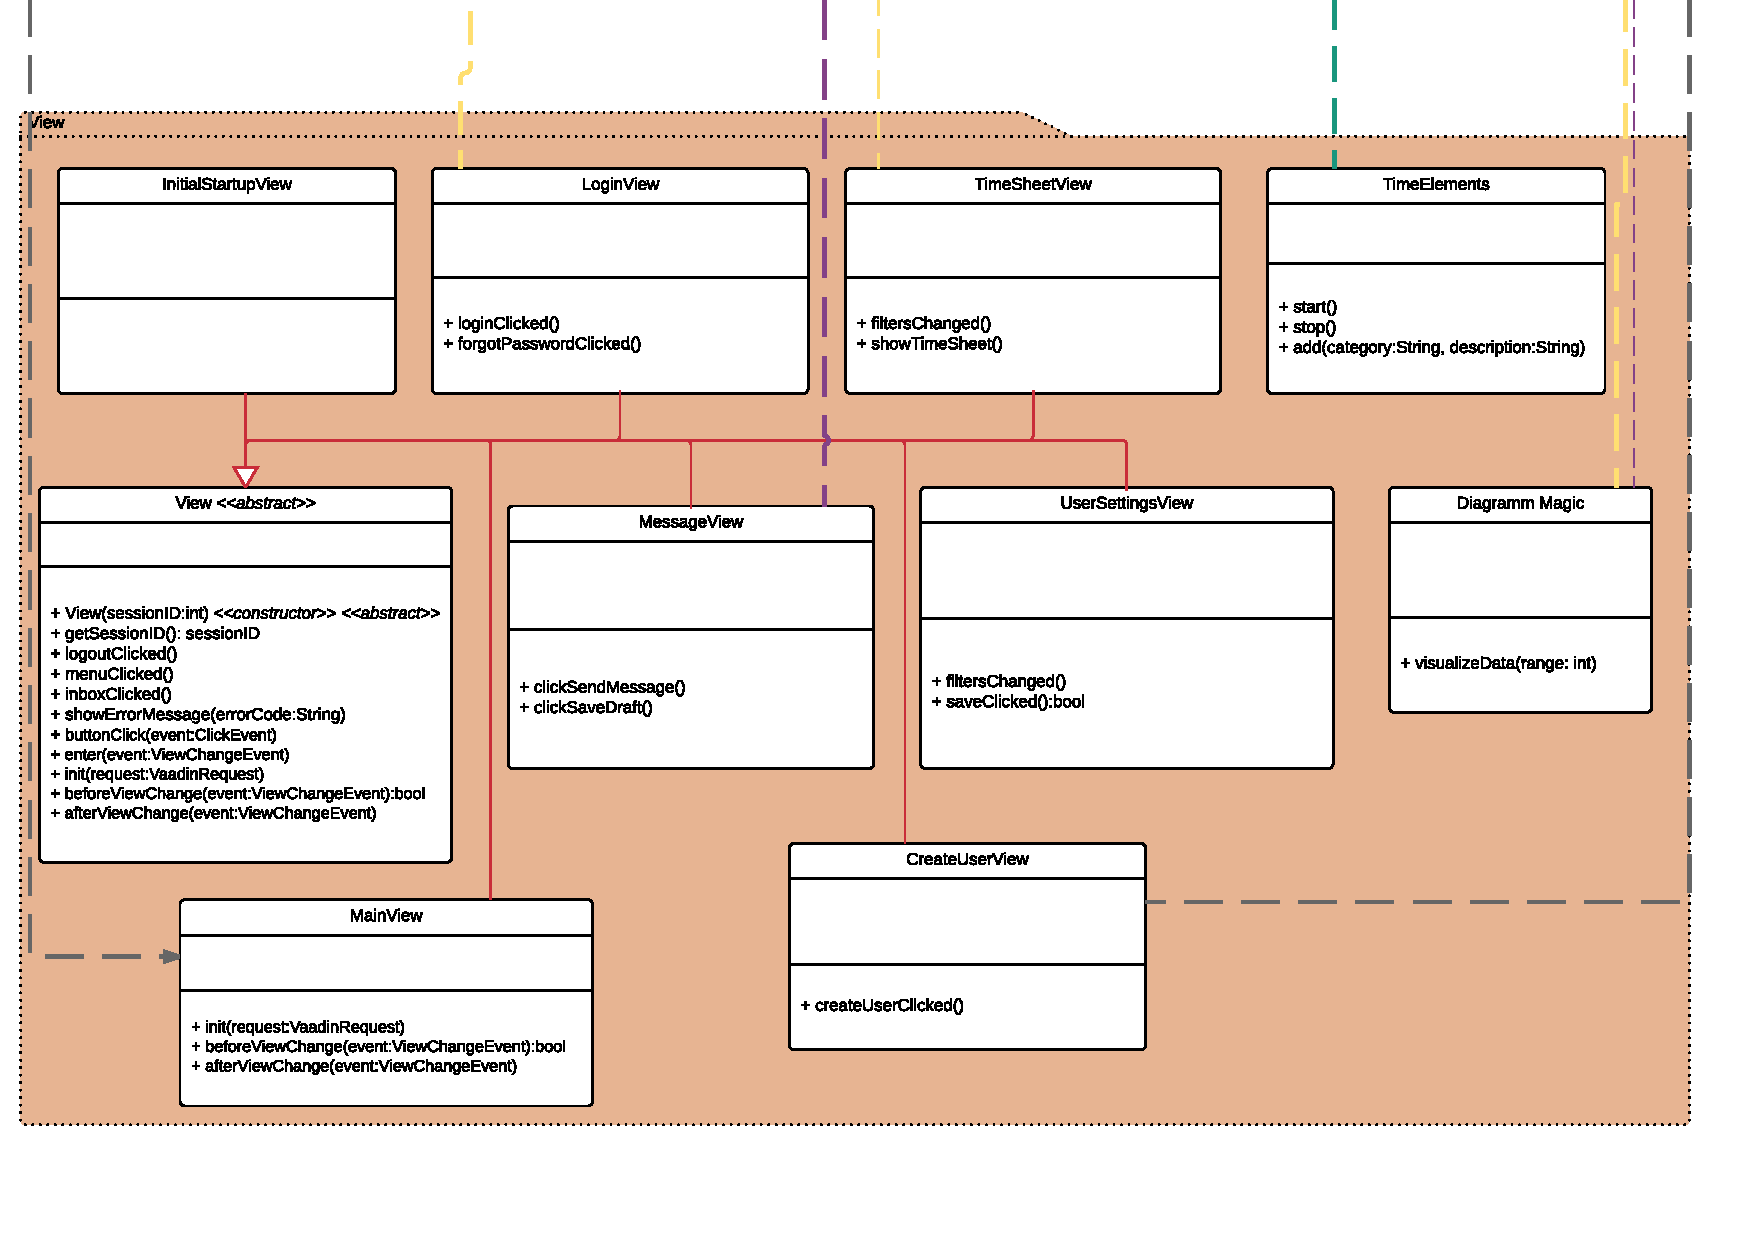
\includegraphics[width=\linewidth]{Diagramms/class/view.pdf}\\
        \begin{itemize}
            \itm{View}
                \emph{Erbende Klassen:}
                \begin{itemize}

                    \itm{InitialStartupView}

                    \itm{LoginView}
                    \begin{itemize}
                        \itm{loginPressed()}
                        \itm{}
                    \end{itemize}

                    \itm{TimeSheetView}
                    \begin{itemize}
                        \itm{filtersChanged()}
                        \itm{showTimeSheet()}
                    \end{itemize}

                    \itm{UserSettingsView}
                    \begin{itemize}
                        \itm{filtersChanged()}
                        \itm{}
                    \end{itemize}

                    \itm{MainView}
                    \begin{itemize}
                        \itm{LoadView(sessionID:int)}
                    \end{itemize}

                    \itm{MessageView}
                    \begin{itemize}
                        \itm{clickSendMessage()}
                        \itm{clickSaveDraft()}
                    \end{itemize}

                    \itm{CreateUserView}
                    \begin{itemize}
                        \itm{createUserClicked()}
                    \end{itemize}

                \end{itemize}
                \begin{itemize}
                    \itm{View(sessionID:int)}
                    \itm{getSessionID(): sessionID}
                    \itm{logoutClicked()}
                    \itm{menuClicked()}
                    \itm{inboxClicked()}
                    \itm{showErrorMessage(errorCode:String)}
                    \itm{buttonClick(event:ClickEvent)}
                    \itm{enter(event:ViewChangeEvent)}
                    \itm{init(request:VaadinRequest)}
                    \itm{beforeViewChange(event:ViewChangeEvent):bool}
                    \itm{afterViewChange(event:ViewChangeEvent)}
                \end{itemize}

            \itm{Diagramm Magic}
            \begin{itemize}
                \itm{visualizeData(range: int)}
                    Zeigt die Daten aus der StatisticControl an.
            \end{itemize}

            \itm{TimeElements}
            \begin{itemize}
                \itm{start()}
                \itm{stop()}
                \itm{add(category:String, description:String)}
            \end{itemize}

        \end{itemize}

    \subsection{Entwurfsmuster}
        \begin{itemize}
            \item Die Klasse GermanLawRegulations implementiert zusammen mit Regulations und RegulationControl das Strategie-Entwurfsmuster.
                Dies macht es einfacher, Gesetze von anderen Ländern zu implementieren und zu benutzen.
            \item Alle auf DAO endenden Klassen implementieren das Fabrik-Entwurfsmuster, um auf in der Datenbank abgelegte Klassen zuzugreifen.
                Damit wird der Zugriff auf die Datenbank von den anderen Klassen abgekapselt.
            \item Jede der von Control erbenden Klassen implementiert das Singleton-Entwurfsmuster, da die Klassen keine Zustände haben und nicht bei jeder Benutzung neu initialisiert werden müssen.
            \item Jede der von View erbenden Klassen bildet zusammen mit View das Schablenenmethode-Entwurfsmuster, da das Vaadin-Framework dies so vorgibt.
        \end{itemize}
